\chapter{Appendix}\label{ch:appendix}

\section{Implementation of Special Kernel Features}\label{sec:9-special-kernel-features}

RME can support many special features provided by certain other operating systems, such as CPU hotplug, memory hotplug, the separation kernel, para-virtualization, and so on. Their implementation ideas are briefly described below.

\subsection{Implementation of CPU Hotplug}\label{subsec:9-cpu-hotplug}

CPU hotplug is divided into two functions. One is hot plug-in, that is, inserting a new CPU to increase the number of CPUs; the other is hot plug-out, that is, pulling a CPU out of its socket to decrease the number of CPUs. RME's support for this feature depends on the hardware-level support provided by the underlying hardware platform, and both must be accomplished with customized kernel function calls.

For hot plug-in, after the insertion of a physical CPU package is detected, the processor can be initialized and the required Init threads can be created, after which these processor cores can be used.

Hot plug-out is the opposite: the activities of the corresponding processor must be stopped, and the other processor cores must no longer send IPIs to that processor. Only then can we remove this physical CPU package.

\subsection{Implementation of Memory Hotplug}\label{subsec:9-memory-hotplug}

Memory hotplug is likewise divided into two parts: one part is adding memory, and the other part is removing memory. RME's support for this feature depends on the hardware-level support provided by the underlying hardware platform, and it too must be accomplished with customized kernel function calls.

In the case of adding memory, if user-mode memory is being added, it suffices to add the physical page frames corresponding to this memory to some user page table. If kernel memory needs to be added, then the other processors must first be paused, after which new pages are added to the kernel page table and the kernel page table is modified to reflect this change, and finally the other processors are resumed. After all operations are completed, a TLB flush operation must also be performed.

In the case of removing memory, if user-mode memory is being removed, the user-mode library must confirm that these physical pages are not currently mapped. At this point, the mappings of these pages can be removed directly and the memory module can be pulled out. If kernel memory is being removed, then the other processors must first be paused, after which the data in the memory to be removed is copied onto blank physical pages and the kernel page table is modified to reflect this change, and finally the other processors are resumed. After all operations are completed, a TLB flush operation must also be performed.

\subsection{Implementation of the Separation Kernel}\label{subsec:9-isolated-kernel}

Because RME is a microkernel operating system, it is very convenient, just like Barrelfish\hyperref[cite:9-1]{{[}1{]}}, to run multiple instances of RME on a single physical machine. Each instance can manage one or more CPU cores, and communication can then be implemented in user mode through shared memory or a network among the multiple operating systems. This approach does not require the caches among CPUs to be coherent, does not require the features contained in each CPU to be the same, and does not even require the instruction sets and architectures of the CPUs to be the same. If processors of multiple architectures are used in such a system, then RME and the user-mode library need to be ported separately for them.

\needspace{14\baselineskip}
For example, if there is a SoC or single-board computer as shown in the figure below\footnote{HMMU refers to a hardware-filled MMU, and SMMU refers to a software-filled MMU}, then it is possible to run RME on all of the cores, and then accomplish information transfer through shared memory among the different subsystems.

\begin{figure}[H]
    \centering
    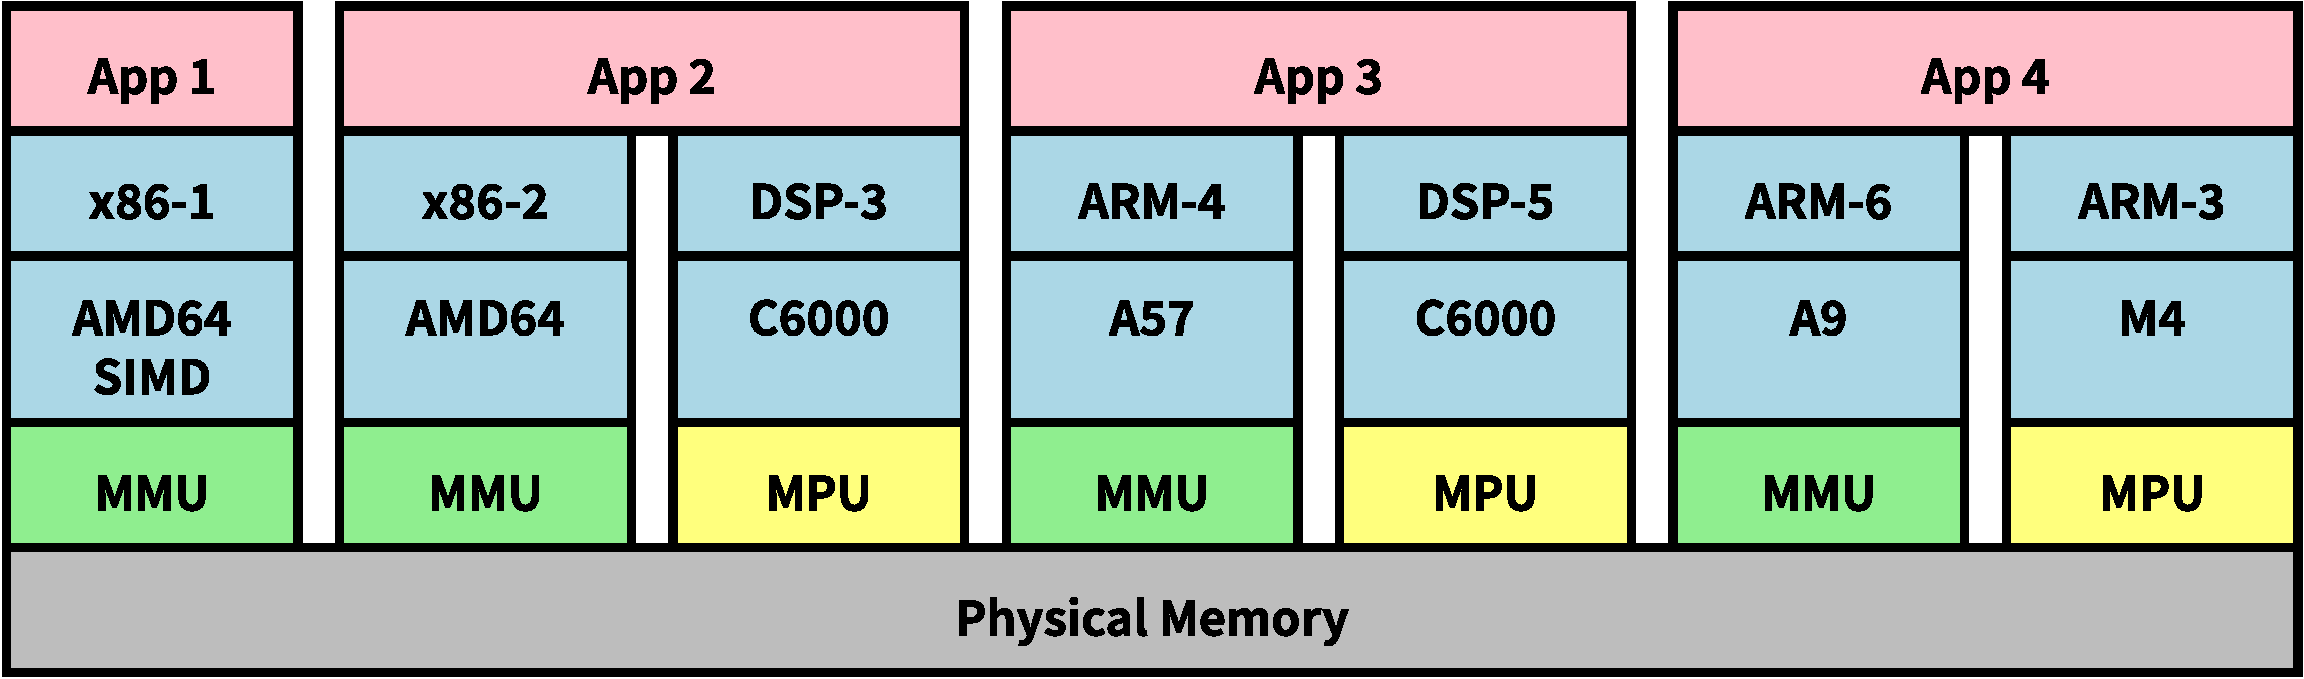
\includegraphics[width=0.72\textwidth]{Figure/image14.pdf}
    \caption{Typical Implementation of a Heterogeneous Multi-core Separation Kernel}
    \label{fig:9-1-heterogeneous-multicore-isolated-kernel}
\end{figure}

\needspace{14\baselineskip}
The figure above shows an example in which different architectures run together. It is also feasible to run one instance of RME on each different NUMA node, as shown in the following figure:

\begin{figure}[H]
    \centering
    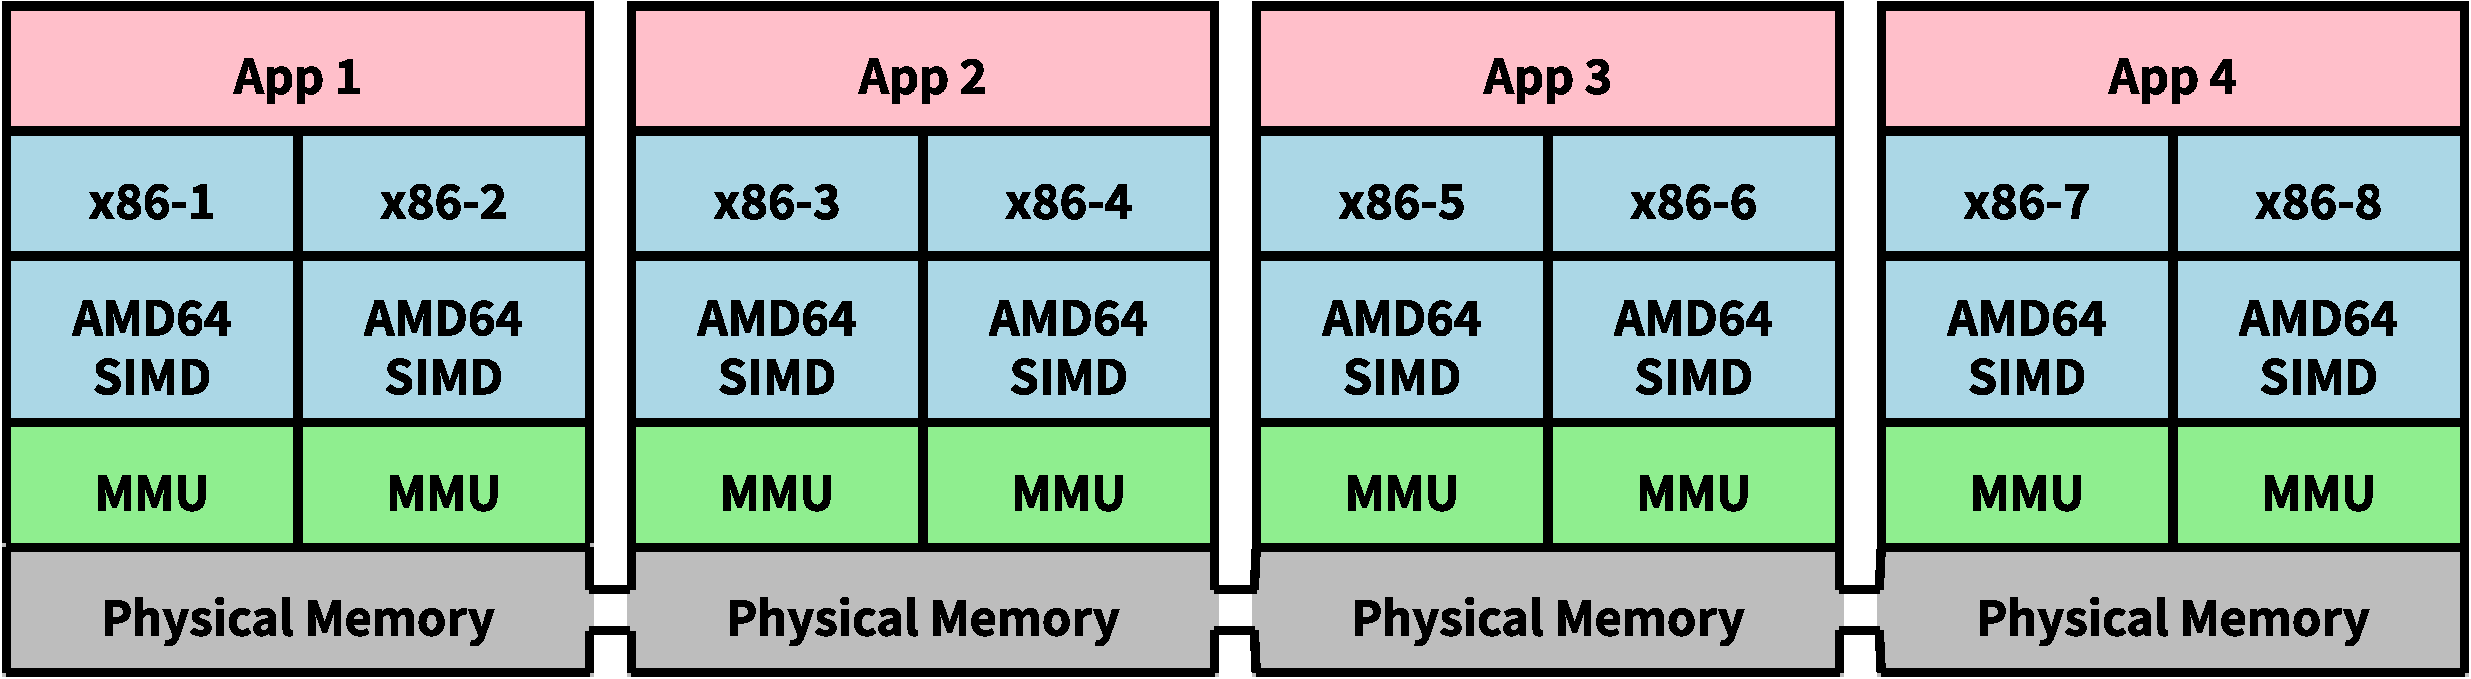
\includegraphics[width=0.72\textwidth]{Figure/image15.pdf}
    \caption{Typical Implementation Scheme of a Separation Kernel Based on NUMA}
    \label{fig:9-2-numa-isolated-kernel}
\end{figure}

\subsection{Implementation of a Tickless Kernel}\label{subsec:9-tickless-kernel}

A tickless kernel requires that every CPU core of the system have an independently programmable high-precision timer, and that this high-precision timer generate a variable scheduler timer interrupt. The ratio between a timeslice and the timer reload value can be freely decided by the implementer as needed. To facilitate the implementation of a tickless kernel, the system provides two functions, \_RME\_Tim\_Future and \_RME\_Tim\_Elapse; they may be ignored if a tickless kernel is not implemented.

In order for the timer to generate an interrupt at the potential next timeout point, after every change of the remaining timeslice of the current thread\footnote{such as at the exit of the various interrupt vectors}, this time must be set as the next timeout time of the hardware timer. Three situations may cause the remaining timeslice to change: (1) a context switch caused by any reason\footnote{There is also the coincidence that the remaining timeslices of the threads before and after the context switch are exactly the same; in this case the timer does not need to be reprogrammed}, (2) RME\_SVC\_THD\_TIME\_XFER is used in the system call vector and the timeslice of the current thread changes as a result, and (3) a timer interrupt occurs\footnote{The occurrence of this interrupt does not necessarily mean that a thread has exhausted its own timeslice; it may also mean that the longest configurable timeout of the hardware timer is not long enough, so that one timing period must be completed in several segments}. On some architectures, reprogramming the timer may take a relatively long time, and the occurrence of an interrupt does not necessarily cause the remaining timeslice to change, so one may query and determine the change of the current thread's timeslice before and after entering the interrupt by oneself to decide whether the timer needs to be reprogrammed; the timer interrupt is a special case, since it definitely requires one timer reprogramming, and thus this query can be omitted.

The kernel provides the function \_RME\_Tim\_Future to obtain this timeout time. If the length of this period exceeds the range that the hardware timer can support, it suffices to set the timeout time of the hardware timer to the maximum allowed value; the design of RME guarantees that only the time that has actually elapsed is deducted from the remaining time of the thread, so there is no need to worry about the loss of the thread's remaining time.

\begin{xltabular}{\textwidth}{@{}>{\hsize=0.5279\hsize\raggedright\arraybackslash}X>{\hsize=1.4721\hsize\raggedright\arraybackslash}X@{}}
\caption{Obtaining the Number of Timeslices Until the Nearest Timeout}\label{tab:9-1-latest-timeout-slices}\\
\toprule
Prototype & rme\_ptr\_t \_RME\_Tim\_Future(void)\tabularnewline
\endfirsthead
\toprule
Prototype & rme\_ptr\_t \_RME\_Tim\_Future(void)\tabularnewline
\midrule
\endhead
\bottomrule
\endlastfoot
Meaning &
The number of timeslices from now to the nearest future timeout; the next timeout time of the system timer can be set according to this value.\tabularnewline
Return value\strut
 & rme\_ptr\_t

The number of timeslices from now to the nearest future timeout.\strut
\tabularnewline
Parameters & None.\tabularnewline
\end{xltabular}
\nopagebreak[4]

In order for the time consumed by all threads to be precisely recorded, the time already consumed must be deducted from the current thread before every point at which a context switch may occur or the timeslice may be modified\footnote{At the entry of every interrupt vector except the timer interrupt (which calls \_RME\_Tim\_Handler); strictly speaking, if it can be determined that this interrupt does not cause a thread switch and does not modify the timeslice of the current thread through RME\_SVC\_THD\_TIME\_XFER, then there is no need to call \_RME\_Tim\_Elapse, but determining whether a thread switch occurs is very difficult, and the overhead of \_RME\_Tim\_Elapse is very low, so it is recommended to call it at the entry of all interrupt vectors}. The kernel provides the function \_RME\_Tim\_Elapse for this purpose to record the consumed time.

\begin{xltabular}{\textwidth}{@{}>{\hsize=0.5279\hsize\raggedright\arraybackslash}X>{\hsize=1.4721\hsize\raggedright\arraybackslash}X@{}}
\caption{Recording the Elapsed Time}\label{tab:9-2-record-elapsed-time}\\
\toprule
Prototype & void \_RME\_Tim\_Elapse(rme\_ptr\_t Slice)\tabularnewline
\endfirsthead
\toprule
Prototype & void \_RME\_Tim\_Elapse(rme\_ptr\_t Slice)\tabularnewline
\midrule
\endhead
\bottomrule
\endlastfoot
Meaning &
Records the number of timeslices already used by the current thread before initiating a potential context switch.\tabularnewline
Return value & None.\tabularnewline
Parameters\strut
 & rme\_ptr\_t Slice

The number of timeslices that have elapsed since the last call to \_RME\_Tim\_Elapse or \_RME\_Tim\_Handler.\strut
\tabularnewline
\end{xltabular}
\nopagebreak[4]

It is worth noting that although a tickless kernel has lower CPU power consumption, its real-time performance is not necessarily better, because it inevitably includes the registration of elapsed time before a context switch and the reprogramming of the timer after a context switch. Both may increase the length of the context switch critical section and negatively affect the real-time performance of the system. Moreover, the signal that the kernel sends to the timer endpoint will also lose its periodicity, and user mode can no longer rely on it.

When a tickless kernel is used, the RME\_TIMESTAMP macro must be defined as a read of some independent one-way incrementing counter\footnote{Such a counter can usually be found in the CPU performance monitoring unit (Performance Monitoring
  Unit, PMU) or in a global timer; some architectures such as x86 also provide a dedicated RDTSC instruction that increments constantly (CONSTANT\_TSC) and never stops (NONSTOP\_TSC)}, which makes the timestamp the globally latest value at all times, thereby guaranteeing the safety of the quiescence period of capability operations.

\subsection{Implementation of Processor Sleep}\label{subsec:9-processor-sleep}

Processor sleep is notoriously difficult to implement correctly; a careless design may in mild cases cause lost wakeups and system stalls, and in severe cases cause permanent sleep and a machine freeze. The definitions of the sleep instruction adopted by processors can be divided into the ``look-before-and-after'' type, the ``after-only'' type, and the ``trigger-only'' type, and the three definitions differ greatly in implementation strategy. If there is concern that sleep cannot be implemented correctly, it can be omitted. The system's power consumption will be slightly higher; this is the only cost of not sleeping.

\subsubsection{The ``Look-Before-and-After'' Type}\label{subsubsec:9-sleep-look-before-and-after}

This is the sleep instruction definition that is the most complex in hardware design and the simplest in software use\footnote{such as the WFE instruction of ARMv7-M after SEVONPEND is set}. This kind of sleep instruction behaves in exactly the same way regardless of whether the processor's global interrupt enable is set. It (1) always atomically checks, before execution, whether an interrupt is already pending; if so, it executes as a NOP and does not enter sleep; and (2) always checks, after execution, whether a new interrupt is currently pending or triggered; if so, it immediately exits sleep and resumes instruction execution.

For this type, it suffices to simply execute the sleep instruction when sleeping; there is no need to worry about lost interrupt wakeups.

\subsubsection{The ``After-Only'' Type}\label{subsubsec:9-sleep-after-only}

This is a sleep instruction definition that is relatively complex in both hardware design and software use\footnote{such as the WFI instruction of some non-standard RISC-V processors; the standard WFI instruction is of the ``look-before-and-after'' type}. This kind of sleep instruction behaves in exactly the same way regardless of whether the processor's global interrupt enable is set. Unlike the ``look-before-and-after'' type, however, it does not check before execution whether an interrupt is already pending; it only checks after execution whether a new interrupt is currently pending or triggered, and if so, it immediately exits sleep and resumes instruction execution.

For this type, executing it with interrupts disabled requires vigilance against lost interrupt wakeups. If no special handling is performed and a new interrupt becomes pending after interrupts are disabled but before the sleep instruction is executed, the wakeups from these pending interrupts may be lost. A naive approach is to first determine whether there is a pending interrupt and enter sleep only if there is none: if no interrupt is pending at the time of the check, but a new interrupt becomes pending after the check has finished and before sleep is executed, the wakeup from this newly arrived interrupt will likewise be lost.

If lost interrupts are not a concern, it suffices to simply execute the sleep instruction when sleeping. If lost interrupts cannot be tolerated, it must be handled as the ``trigger-only'' type described in the next subsection. However, some processors have a configuration switch that converts the behavior of the sleep instruction into the ``look-before-and-after'' type described in the previous subsection; if such a switch can be found, it can simply be turned on.

\subsubsection{The ``Trigger-Only'' Type}\label{subsubsec:9-sleep-trigger-only}

This is the sleep instruction definition that is the simplest in hardware design but the most complex in software use\footnote{such as the HALT instruction of x86}. This kind of sleep instruction can only be used when the processor's global interrupt enable is set, and once it is used, the processor immediately stops and waits for a new interrupt to arrive. If such an instruction is mistakenly executed with interrupts disabled, the processor will lock up because it cannot accept interrupts, causing the machine to freeze permanently. This causes trouble for RME: RME always executes the sleep instruction in the system call interrupt context------where interrupts are necessarily disabled------because the sleep feature is provided through a kernel function call. Monolithic kernels such as Linux do not have this problem, because they have a genuine kernel idle thread with interrupts enabled that is responsible for sleeping.

For this type, we need to forge an environment similar to a Linux ``kernel thread'' in which to invoke the sleep instruction. Specifically:

(1) Write a piece of code as the ``kernel thread'', in which the sleep instruction is called in a loop. It does not need to contain any other content, nor does it need a separate stack.

(2) Once a sleep request is detected in \_RME\_Svc\_Handler, exit the interrupt context to this ``kernel thread'' in assembly\footnote{rather than the usual return to user mode}, and enable interrupts at the same time as exiting to this ``kernel thread''. To this end, a return stack can be forged on the spot; the stack of this ``kernel thread'' still uses the current kernel stack, while the current kernel context is saved onto the current kernel stack.

(3) When the first interrupt after sleeping arrives, check whether the interrupt interrupted the ``kernel thread''. If so, record that this interrupt has occurred, but do not run its interrupt vector for the time being; instead, restore the kernel context and continue the execution of \_RME\_Svc\_Handler. There is no need to be concerned about whether the ``kernel thread'' has finished running.

(4) After \_RME\_Svc\_Handler finishes running, scan the interrupt occurrence record and run the deferred interrupt vectors. Finally, return to user mode in the usual manner.

In this way, the sleep instruction is invoked with interrupts enabled, so a sleep-related lockup will not occur; after the processor is woken up, it continues executing the previous kernel function call, and the interrupt vectors are processed only after that call has been fully handled, so kernel reentrancy will not occur on a uniprocessor.

\subsection{Saving and Restoring the Coprocessor Context}\label{subsec:9-coprocessor-context-switch}

Coprocessors refer to CPU extension modules such as floating-point processors and vector processors, and they also have their own contexts; regardless of whether multiple threads share the same coprocessor, its context must be handled carefully, otherwise, in addition to causing program corruption, it will also turn the coprocessor register set into a huge covert storage channel. This is very different from RMP, which cares only about temporal isolation and not about spatial isolation. In addition, RME has a class of para-virtualization dedicated threads whose register state is untrusted; the coprocessors of such threads need to be handled even more carefully, because the coprocessor state they report is also untrusted.

The main function in charge of coprocessor context switching is \_\_RME\_Thd\_Cop\_Swap, which is introduced in \ref{subsubsec:7-coprocessor-register-set-functions}
and is responsible for saving and restoring the context of the coprocessor together during a thread context switch. The saving and restoration of the coprocessor are implemented in it.

According to the functional model that the processor hardware layer provides for coprocessor control, coprocessors can be classified into the ``always-on'' type, the ``off-on'' type, the ``off-initial-used'' type, and the ``off-initial-clean-dirty'' type, where each provides more control functionality than the preceding one in order to optimize its context switch performance, and its optimal switch strategy is correspondingly more complex. Of course, each type can use the switch strategy of the types preceding it at the cost of performance; when (1) the information security requirements are very high, (2) it is uncertain how the switch strategy should be implemented, or (3) the current strategy implementation is suspected of being wrong, the ``always-on'' switch strategy can be used uniformly.

\subsubsection{The ``Always-On'' Type}\label{subsubsec:9-coproc-always-on}

This is the simplest coprocessor control model. Under this model, if the coprocessor is implemented at the hardware level, it will be permanently on when the hardware is powered up and cannot be turned off, or it is enabled by default in most software environments\footnote{such as the MMX coprocessor of x86; although it has a switch, it is basically standard equipment and can be treated as the ``always-on'' type}. Such a coprocessor is a coprocessor in name only; it can even be treated as part of the general register set, so its switch strategy is self-evident: switch the coprocessor register set at all times. Of course, the context attribute Attr of every thread in the system must contain this coprocessor.

Under this strategy, no special handling of para-virtualization dedicated threads is required.

\subsubsection{The ``Off-On'' Type}\label{subsubsec:9-coproc-on-off}

This is the second simplest coprocessor control model. Under this model, the hardware implements a coprocessor that is off by default at system startup; its switch must be turned on before it can be used, otherwise an exception will be generated\footnote{such as the COP1 floating-point coprocessor of MIPS, which provides a simple on/off control bit}. In this case, the coprocessor context can be switched according to the following strategy:

First, (1) determine whether the context attribute Attr\_Cur of the current thread includes this coprocessor; if it does, turn on the coprocessor and save its context into the current thread's context structure; if it does not, do nothing. Then, (2) determine whether the context attribute Attr\_New of the new thread includes this coprocessor; if it does, turn on the coprocessor and restore the context from the new thread's context structure into the coprocessor; if it does not, turn off the coprocessor.

Under this strategy, no special handling of para-virtualization dedicated threads is required, unless the on/off state of the coprocessor is also reported by a register under its control. Since the coprocessor on/off state it reports is not trustworthy, the final on/off state of the coprocessor should be forcibly kept consistent with the context attribute. This also applies to the subsequent types and will not be repeated below.

It is not recommended to use the ``turn off after switching''-``exception''-``turn on'' cyclic strategy\footnote{Quite a number of operating systems adopt this strategy} on such hardware to implement lazy software saving of the coprocessor state, because this strategy worsens the worst-case execution time: first, coprocessors on all architectures have switch overhead of varying magnitude, and this strategy increases the number of switches; second, if two alternately switched threads both use the coprocessor frequently, then each thread switch generates an additional coprocessor enable exception. In fact, the saving of the coprocessor state can be postponed until the last moment------for example, until just before the new thread begins to use the coprocessor, or until just before the coprocessor state structure of the current thread must be updated\footnote{Those kernel function calls that query registers may read the coprocessor state}------and only then performed, but this requires recording which thread the current coprocessor state belongs to and tracking it at all times, which imposes an additional mental burden on the porter. This may be done only when average performance is far more important than the worst-case execution time, and when doing so one must have a clear understanding of the speculative execution (Speculative
execution) mechanism of the processor microarchitecture, otherwise it may cause leakage of the coprocessor state\footnote{To avoid this situation, official ports never use one thread's coprocessor context to execute another thread, even if the coprocessor is off}.

However, it is encouraged to use the ``initially off''-``first exception''-``permanently on'' strategy to convert such hardware into the ``off-initial-dirty'' type and adopt its ``switch strategy 1'', because the exception is raised only once, when a thread first uses the coprocessor.

\subsubsection{The ``Off-Initial-Dirty'' Type}\label{subsubsec:9-coproc-off-initial-dirty}

This is a relatively common coprocessor control model. Under this model, the hardware not only implements a coprocessor switch, but also detects in real time whether the coprocessor has been used. If the coprocessor is not turned on, using it generates an exception; if the coprocessor is turned on but has not actually been accessed, the ``dirty'' bit will not be set by the hardware until the coprocessor is actually accessed for the first time\footnote{such as the FPv4 and FPv5 floating-point processors of ARMv7-M}. In this case, there are two handling strategies for the context of this coprocessor:

The first strategy treats the ``dirty'' bit as an indication of the ``initial state''. It is the most commonly used strategy; it helps to skip unnecessary context saving and restoration for threads that declare the coprocessor in their context attributes but have never touched it\footnote{It should be declared as used even if the thread does not use the coprocessor throughout its entire lifetime, which helps to improve forward compatibility}, and it is the strategy used in the official ports of RME; this strategy is similar to the strategy adopted by RMP. The specific operations of this strategy are shown in the following table.

\begin{xltabular}{\textwidth}{@{}>{\hsize=0.9261\hsize\raggedright\arraybackslash}X>{\hsize=0.6708\hsize\raggedright\arraybackslash}X>{\hsize=1.4031\hsize\raggedright\arraybackslash}X@{}}
\caption{``Off-Initial-Dirty'' Type Switch Strategy 1}\label{tab:9-3-off-initial-dirty-strategy-1}\\
\toprule
Current thread & New thread & Operation\tabularnewline
\endfirsthead
\toprule
Current thread & New thread & Operation\tabularnewline
\midrule
\endhead
\bottomrule
\endlastfoot
\multirow{3}{=}{\parbox{\hsize}{\raggedright\hyphenpenalty=10000 Does not include the coprocessor (not in Attr)}} & Does not include the coprocessor\strut
 & Nothing needs to be done\strut
\tabularnewline
& Coprocessor untouched & Turn on the coprocessor\tabularnewline
& Coprocessor used &
Turn on the coprocessor and restore the coprocessor context from the new thread's context structure\tabularnewline
\multirow{3}{=}{\parbox{\hsize}{\raggedright\hyphenpenalty=10000 Coprocessor untouched (initial)}} & Does not include the coprocessor\strut
 & Turn off the coprocessor\strut
\tabularnewline
& Coprocessor untouched & Nothing needs to be done\tabularnewline
& Coprocessor used &
Restore the coprocessor context from the new thread's context structure\tabularnewline
\multirow{3}{=}{\parbox{\hsize}{\raggedright\hyphenpenalty=10000 Coprocessor used (dirty)}} & Does not include the coprocessor\strut
 & First save the coprocessor context into the current thread's context structure, then reinitialize the coprocessor context, and finally turn off the coprocessor\strut
\tabularnewline
& Coprocessor untouched &
Save the coprocessor context into the current thread's context structure and reinitialize the coprocessor context\tabularnewline
& Coprocessor used &
Save the coprocessor context into the current thread's context structure and restore the coprocessor context from the new thread's context structure\tabularnewline
\end{xltabular}
\nopagebreak[4]

Under this strategy, special vigilance is required against para-virtualization dedicated threads, because the ``dirty'' bit they report is not reliable. After modifying the coprocessor context, such a thread can clear the ``dirty'' bit in user mode to report a forged ``initial state''\footnote{This situation occurs only when multiple CPU cores are present; other cores can modify this data structure in parallel}, and can thereby leak its own coprocessor state to the new thread. Therefore, as long as the current thread is a para-virtualization dedicated thread, its ``dirty'' bit state must be ignored and it must be considered to have used the coprocessor. However, when it reports that it is in the ``initial state'', it is not necessary to save the coprocessor context into its context structure; this does not harm honest para-virtualization dedicated threads.

The second strategy treats the ``dirty'' bit as an indication that the context ``has been saved''. It helps to skip unnecessary context saving during execution segments in which the coprocessor is not used by threads that use the coprocessor intermittently, and can improve average performance when all threads actually use the coprocessor, but it provides no benefit for the worst-case execution time. The specific operations of this strategy are shown in the following table.

\begin{xltabular}{\textwidth}{@{}>{\hsize=0.7814\hsize\raggedright\arraybackslash}X>{\hsize=1.0349\hsize\raggedright\arraybackslash}X>{\hsize=1.1837\hsize\raggedright\arraybackslash}X@{}}
\caption{``Off-Initial-Dirty'' Type Switch Strategy 2}\label{tab:9-4-off-initial-dirty-strategy-2}\\
\toprule
Current thread & New thread &
Operation\tabularnewline
\endfirsthead
\toprule
Current thread & New thread &
Operation\tabularnewline
\midrule
\endhead
\bottomrule
\endlastfoot
\multirow{2}{=}{\parbox{\hsize}{\raggedright\hyphenpenalty=10000 Does not include the coprocessor (not in Attr)}} & Does not include the coprocessor\strut
 & Nothing needs to be done\strut
\tabularnewline
& Coprocessor saved &
Turn on the coprocessor and restore the coprocessor context from the new thread's context structure\tabularnewline
\multirow{2}{=}{\parbox{\hsize}{\raggedright\hyphenpenalty=10000 Coprocessor saved (clean)}} & Does not include the coprocessor\strut
 & Turn off the coprocessor (and clear the coprocessor context)\strut
\tabularnewline
& Coprocessor saved &
Restore the coprocessor context from the new thread's context structure\tabularnewline
\multirow{2}{=}{\parbox{\hsize}{\raggedright\hyphenpenalty=10000 Coprocessor not saved (dirty)}} & Does not include the coprocessor\strut
 & First save the coprocessor context into the current thread's context structure, then clear the current thread's ``dirty'' bit, and finally turn off the coprocessor (and clear the coprocessor context)\strut
\tabularnewline
& Coprocessor saved &
First save the coprocessor context into the current thread's context structure, then clear the current thread's ``dirty'' bit, and finally restore the coprocessor context from the new thread's context structure\tabularnewline
\end{xltabular}
\nopagebreak[4]

Under this strategy, no special handling of para-virtualization dedicated threads is required\footnote{Under this strategy, the ``dirty'' bit of the new thread is necessarily cleared}. Even if the state of the ``dirty'' bit it reports is not trustworthy, the coprocessor context is always reloaded when switching to it, so it is impossible to leak its own context by maliciously manipulating this bit.

Note: in theory, the operating system can introduce an additional variable in the thread context structure to record the ``initial'' state, which is used to separately indicate whether the thread has ever touched the coprocessor; this can convert the ``off-initial-dirty'' type into the ``off-initial-clean-dirty'' type described in the next subsection to further improve performance. However, this introduces additional complexity and memory consumption, and introducing this variable imposes an additional mental burden on readers of the code, so the official ports of RME do not adopt this scheme.

\needspace{24\baselineskip}
\subsubsection{The ``Off-Initial-Clean-Dirty'' Type}\label{subsubsec:9-coproc-off-initial-clean-dirty}

This is the most advanced and most complex coprocessor control model; it provides native, independent indications for all states of the coprocessor, and thus can achieve the best performance. If the coprocessor is not turned on, using it generates an exception; if the coprocessor is turned on but has not actually been accessed, the coprocessor stays in the ``initial'' state until the coprocessor is actually accessed for the first time\footnote{such as the F, D and Q standard extensions of RISC-V}, at which point the hardware makes the coprocessor enter the ``dirty'' state; after the coprocessor context saving during a thread switch is completed, the software does not change the ``dirty'' state to the ``initial'' state, but to the ``clean'' state; any coprocessor access in the ``clean'' state also causes the hardware to turn the coprocessor into the ``dirty'' state. Its switch strategy is shown in the following table:

\begin{xltabular}{\textwidth}{@{}>{\hsize=0.7464\hsize\raggedright\arraybackslash}X>{\hsize=1.0405\hsize\raggedright\arraybackslash}X>{\hsize=1.2131\hsize\raggedright\arraybackslash}X@{}}
\caption{``Off-Initial-Clean-Dirty'' Type Switch Strategy}\label{tab:9-5-off-initial-clean-dirty-strategy}\\
\toprule
Current thread & New thread &
Operation\tabularnewline
\endfirsthead
\toprule
Current thread & New thread &
Operation\tabularnewline
\midrule
\endhead
\bottomrule
\endlastfoot
\multirow{3}{=}{\parbox{\hsize}{\raggedright\hyphenpenalty=10000 Does not include the coprocessor (not in Attr)}} & Does not include the coprocessor\strut
 & Nothing needs to be done\strut
\tabularnewline
& Coprocessor untouched & Turn on the coprocessor\tabularnewline
& Coprocessor saved &
Turn on the coprocessor and restore the coprocessor context from the new thread's context structure\tabularnewline
\multirow{3}{=}{\parbox{\hsize}{\raggedright\hyphenpenalty=10000 Coprocessor untouched (initial)}} & Does not include the coprocessor\strut
 & Turn off the coprocessor\strut
\tabularnewline
& Coprocessor untouched & Nothing needs to be done\tabularnewline
& Coprocessor saved &
Restore the coprocessor context from the new thread's context structure\tabularnewline
\multirow{3}{=}{\parbox{\hsize}{\raggedright\hyphenpenalty=10000 Coprocessor saved (clean)}} & Does not include the coprocessor\strut
 & Reinitialize the coprocessor context and turn off the coprocessor\strut
\tabularnewline
& Coprocessor untouched & Reinitialize the coprocessor context\tabularnewline
& Coprocessor saved &
Restore the coprocessor context from the new thread's context structure\tabularnewline
\multirow{3}{=}{\parbox{\hsize}{\raggedright\hyphenpenalty=10000 Coprocessor not saved (dirty)}} & Does not include the coprocessor\strut
 & First save the coprocessor context into the current thread's context structure, then change the current thread to the ``clean'' state, then reinitialize the coprocessor context, and finally turn off the coprocessor\strut
\tabularnewline
& Coprocessor untouched &
First save the coprocessor context into the current thread's context structure, then change the current thread to the ``clean'' state, and finally reinitialize the coprocessor context\tabularnewline
& Coprocessor saved &
First save the coprocessor context into the current thread's context structure, then change the current thread to the ``clean'' state, and finally restore the coprocessor context from the new thread's context structure\tabularnewline
\end{xltabular}
\nopagebreak[4]

Under this strategy, special vigilance is required against para-virtualization dedicated threads, because any coprocessor state they report is not reliable\footnote{Under this strategy, the new thread cannot be in the ``dirty'' state}. After modifying the coprocessor context, such a thread can modify the coprocessor state register in user mode to report a forged ``initial'' state, and can thereby leak its own coprocessor state to the new thread. Therefore, as long as the current thread is a para-virtualization dedicated thread, the ``initial'' state it reports must be treated as the ``clean'' state.

\subsection{Implementation of Direct User-Mode Page Table Management}\label{subsec:9-user-mode-page-table-management}

Although the RME kernel does its utmost to provide efficient abstractions for page tables, out of considerations such as controllable worst-case execution time and maximum user-mode flexibility, each level of page directory in RME corresponds to one capability, so page table operations are fine-grained but inefficient. On the one hand, in microcontroller scenarios where the page table mappings generally do not need to be modified\footnote{The page tables of a memory protection unit are purely software-simulated; if the mappings do not need to be modified, they are not needed at all}, a large number of page directories and their capabilities consume the already limited system memory; on the other hand, in microprocessor scenarios where page tables need to be modified frequently or in large quantities\footnote{This is generally due to page faults, and page faults are the underlying means of implementing lazy requests; in operating systems that care about average performance and resource utilization (such as cloud computing), lazy requests in turn provide the foundational support for a series of efficiency optimizations}, the low efficiency of page table operations drags down the throughput and tail latency of the entire system. Considering that the requirements for memory management differ vastly across scenarios, RME believes that the authority and responsibility for memory management essentially belong to the user\footnote{All performance problems are essentially problems of authority and responsibility}: the user is responsible for implementing page table management itself when its requirements are special.

Defining RME\_PGT\_RAW\_ENABLE as 1 enables the direct user-mode page table management feature. Once this feature is enabled, page table management is fully controlled by a trusted user-mode process, which is essentially part of the kernel\footnote{Compromising it has exactly the same consequences as compromising the kernel; in other words, it belongs to the trusted computing base (Trusted
  Computing Base, TCB)}, and differs from the kernel only in that (1) it ostensibly runs in user mode, and (2) for the preceding reason, it can be preempted and therefore does not affect the worst-case execution time of the system. In this case, the page-table-related system calls and related low-level functions change somewhat; for these changes, please refer to \ref{subsec:7-general-macro-definitions},
and they will not be repeated here. The design of direct user-mode page table management in extreme scenarios will be elaborated in the next two subsections.

\subsubsection{Deeply Embedded Scenarios}\label{subsubsec:9-deep-embedded-scenario}

The devices most commonly used in deeply embedded scenarios are microcontrollers (MCUs), whose systems are characterized by dedication to a single purpose, real-time reliability, limited budgets, and tight resources; once a process is created, its address space mappings are basically not modified. In this case, unless the dynamic page feature is to be implemented\footnote{Some RISC-V microcontrollers adopt simplified microarchitectures for cost reasons and cannot generate precise memory access permission exceptions, and therefore cannot use the dynamic page feature; in this case, there is basically no reason not to enable direct user-mode page table management}, the significance of retaining the page directory data structure and its capabilities is very limited.

In deeply embedded scenarios, the recommended approach is to generate, at project compile time, tables that can be directly filled into the memory protection unit (MPU), and to initialize the MPU directly with these tables during system initialization so as to completely eliminate the kernel page table overhead; these tables are all constants and can therefore be placed in ROM to further reduce memory usage. In addition, this method can generate configuration data tailored to the characteristics of the MPU, and can adapt to a base-address-length MPU better than a path-compressed page table. The RVM virtual machine monitor that accompanies RME provides this feature; for how to enable this feature, please refer to the RVM manual.

\subsubsection{Cloud-Native Service Scenarios}\label{subsubsec:9-cloud-native-scenario}

Compared with deeply embedded scenarios, cloud-native service scenarios are the other extreme; the leading role is played by standard rack-mounted servers based on microprocessors. They often have memory on the order of terabytes, so the memory space occupied by page tables is negligible. However, (1) microprocessor systems are highly dynamic: processes are created and destroyed and memory is allocated and freed very frequently, and the resulting page table operations are large-scale; sometimes hundreds of thousands or even millions of pages are mapped or unmapped at once. If a page table capability operation were required for every page mapping or unmapping, the resulting performance overhead would be non-negligible. Moreover, (2) a page directory must be zeroed by the kernel when it is created, which greatly slows down the kernel's worst-case execution time; if multiple page directories are created in succession, dense jitter may be introduced, thereby causing the tail latency to exceed the limit\footnote{On the client side this often manifests as program stutter and an unresponsive mouse, while on the server side it often manifests as large response fluctuations and poor service quality}. In addition, (3) page faults also introduce an enormous number of page table operations; even on systems with ample memory that do not use page swapping algorithms, page faults play a huge role in deferring data copies and synchronizing data on demand\footnote{For example, the fork call of Linux tries its best to defer the memory copy until the corresponding page is actually modified; a similar mechanism also exists in mmap}, so responding to them swiftly is still very necessary. Finally, (4) it is difficult to decide how much kernel-dedicated memory a server system should allocate, so its kernel object table Kotbl always covers the entire memory range; in this case, the dynamic demarcation between kernel memory and user memory, as well as the management of kernel objects, already require a trusted user-mode process to take care of everything, and adding a page table management feature on top of that is only natural.

The recommended practice in cloud-native service scenarios has no fixed rule, but the general principles are (1) to reduce the number of IPCs for the same amount of page table operation work, (2) to integrate page tables and other memory objects into easy-to-use coarse-grained entities and provide them to applications, (3) to avoid adding one layer after another when multiple management levels exist, and (4) to fully take the temporal and spatial isolation between processes into account when designing mechanisms. Of course, if the address space is not frequently operated on or there are no stringent performance requirements, there is nothing inappropriate about not using direct user-mode page table management.

\section{Recommended Handling Scheme for the Memory Protection Unit}\label{sec:9-mpu-recommendations}

Memory protection units differ considerably among processors. These differences can be divided into three aspects: influence, region organization, and region format; the ways to deal with them are discussed in the following three subsections respectively.

\subsection{Influence of the Memory Protection Unit}\label{subsec:9-mpu-influence}

The difference in this aspect lies in whether the region attributes of the memory protection unit take effect for kernel mode.

\subsubsection{All-Mode-Affecting Type}\label{subsubsec:9-mpu-all-mode-affecting}

This is the most common type of memory protection unit\footnote{such as ARMv7-M}, whose region attributes take effect for both kernel mode and user mode. This means that if the region attributes are not modified when entering the kernel, the access control restrictions and cache policies that user mode applies to certain memory regions will be imposed on the kernel. Once a driver in the kernel\footnote{RME does not encourage this, but when there are extreme real-time requirements it may be necessary to write a small part of the driver into a kernel-mode interrupt vector} needs to access these regions, it may be subject to random and unexpected restrictions\footnote{This depends on which process was interrupted before the interrupt vector was triggered}, thereby causing a kernel failure.

In this case, the recommended approach is to turn off the memory protection unit after entering the kernel, and to turn it on just before leaving the kernel. There is no need to worry that turning off the memory protection unit will cause a kernel failure; this type of memory protection unit has a background region, and when the memory protection unit is off or does not include a certain region, kernel mode will instead use the access permissions of this background region.

All official ports of RME adopt the practice of temporarily turning off the memory protection unit. This means that the kernel always uses the background region when running, and its access permissions and cache policies are the same as when the memory protection unit is not enabled; this is very conducive to porting interrupt vectors in bare-metal drivers.

\subsubsection{User-Mode-Only Type}\label{subsubsec:9-mpu-user-mode-only}

This is the second most common type of memory protection unit; its regions can be configured to take effect only for user mode. Once the kernel is entered, all memory accesses are no longer restricted by it.

In this case, the ideal behavior is obtained without any special handling.

\subsection{Region Organization of the Memory Protection Unit}\label{subsec:9-mpu-region-organization}

The difference in this aspect lies in whether the memory protection unit prepares different regions for different types of memory.

\subsubsection{Unified Type}\label{subsubsec:9-mpu-unified}

The vast majority of processors adopt this design; any of its entries can be assigned to a memory region of any type.

In this case, the ideal behavior is obtained without any special handling.

\subsubsection{Separate Type}\label{subsubsec:9-mpu-separate}

A small number of processors adopt this design; their entries are divided into three parts: code, data and device, each having a certain number of dedicated entries.

RME and RVM currently do not support this design, and RME does not provide a corresponding official port. In fact, none of the microcontroller architectures that RME supports or plans to support include the separate design.

\subsection{Region Format of the Memory Protection Unit}\label{subsec:9-mpu-region-format}

The difference in this aspect lies in the format of the individual regions in the memory protection unit.

\subsubsection{Power-of-Two Type}\label{subsubsec:9-mpu-power-of-two}

This is the most common memory protection unit region format\footnote{such as ARMv7-M}. This format stipulates that the length of the memory area corresponding to each region must be a power of 2, and that the start address of this memory region must be aligned to this power of 2. Some designs also allow a region to be divided equally into 4, 8 or 16 independent subregions, each of which can be selectively enabled or disabled.

This region format is close to the ``page'' of a paged memory management unit, so these regions can be regarded as a software-filled TLB. The path-compressed page table algorithm built into RME copes well with this format.

\subsubsection{Contiguous Type}\label{subsubsec:9-mpu-contiguous}

This is the second most common memory protection unit region format\footnote{such as ARMv8-M}. This format stipulates that an arbitrary start address and end address can be specified for each region, as long as these addresses are aligned to the processor word length.

This region format is close to the ``segment'' of a segmented memory management unit, so the path-compressed page table algorithm built into RME does not match it well. Therefore, when porting, it is recommended to merge consecutive page mappings into the same region; to facilitate such merging by the kernel, user mode should deliberately map consecutive pages in address order.

\subsubsection{Variable}\label{subsubsec:9-mpu-variable}

This is the least common memory protection unit region format\footnote{such as RISC-V}. This format specifies that each logical region can be either power-of-two or contiguous: when the logical region is power-of-two, it occupies one physical region; when the logical region is contiguous, it occupies two physical regions. The total number of physical regions is limited.

This region format is very flexible, so great care must be taken when designing the metadata cache. To maximize the utilization of physical regions as much as possible, when adding contiguous pages, consideration can be given to merging three or more power-of-two logical regions into a single contiguous logical region; this kind of merging may also have to be performed when adding dynamic pages. To make it convenient for the kernel to perform such merging, user mode should intentionally map contiguous pages in address order.

\section{Factors Limiting Multicore Scalability in RME}\label{sec:9-multicore-scalability-limits}

In RME, not all operations can be executed without affecting each other. A typical operation that cannot be executed in this way is multiple CPUs attempting to simultaneously create kernel objects in the same piece of memory. The operations that cannot be executed in parallel are listed below, together with their reasons.

\subsection{Update of RME\_TIMESTAMP}\label{subsec:9-timestamp-update}

If RME\_TIMESTAMP is defined as a variable, its update must be performed by one processor rather than multiple processors. On multicore processors, the other cores need to synchronize this variable into their own cache lines. Therefore, this operation cannot be parallelized well. However, this does not greatly affect the degree of parallelism of the system, because the clock interrupt frequency of large systems can be configured to be relatively low.

If RME\_TIMESTAMP is defined as a read of some free-running counter\footnote{such as the x86 RDTSC}, then this problem does not exist. It is worth noting multi-package systems: although the counters of the cores within the same physical CPU package may be consistent, the counters between different physical CPU packages may become inconsistent. In this case, the porter must solve this problem themselves.

\subsection{Multiple Cores Simultaneously Creating Kernel Objects in the Same Kernel Memory Region}\label{subsec:9-concurrent-kernel-object-creation}

Since the creation of kernel objects always involves writing to the kernel object registry table, when multiple CPUs attempt to concurrently write to the same location in the table, a large number of cache line updates occur, making this operation not parallelize well.

\subsection{Multiple Cores Simultaneously Sending Signals to the Same Signal Endpoint}\label{subsec:9-concurrent-signal-sending}

Since this is an atomic compare-and-swap operation, the CPU and the bus controller may lock the bus at the hardware level, so simultaneous accumulation by multiple cores is actually completed serially. Therefore, this case cannot be parallelized well. Of course, if the system has hardware that can perform accumulation in parallel\footnote{common modern architectures generally have such hardware}, then this problem does not exist.

\subsection{Multiple Cores Simultaneously Performing Capability Transfer or Removal on the Same Root Capability}\label{subsec:9-concurrent-root-capability-transfer}

Since the reference count of a capability is kept inside the root capability, multiple capability transfers or removals performed simultaneously on the same root capability will modify the reference count at the same time. This causes a large number of cache line updates and makes this operation not parallelize well. However, this problem generally does not exist in systems, first because capability transfer is usually a relatively rare operation, and second because in multicore systems user programs usually create dedicated kernel objects for each core.

Since the root capabilities of kernel memory capabilities (RME\_CAP\_TYPE\_KOM) and kernel function call capabilities (RME\_CAP\_TYPE\_KFN) are created only at system boot, any leaf capability of these two types in the system must come from the initial capabilities created at boot, which cannot be deleted. Fortunately, neither of these two types of capabilities has a kernel object, nor are they referenced by any other kernel object, so RME applies a special optimization to them: they do not record their own root capability and do not perform reference counting, thus avoiding this problem.

\section{Factors Limiting RME on 32-Bit Systems}\label{sec:9-32bit-limitations}

In the case of 32-bit processors, RME is constrained by the processor word length in the implementation of certain functions. The two constrained functions are thread creation and quiescence period calculation.

\subsection{A Thread's Thread ID}\label{subsec:9-thread-id}

In RME, each thread corresponds to a TID when it is bound, and its length is half a machine word. Therefore, on a 32-bit system there are only 2\textsuperscript{16} different TIDs in total\footnote{on 64-bit systems this value is 2\textsuperscript{32}, so it is not a problem}. If more threads than this number are to be created, then it means that the TIDs of some threads must overlap when they are bound. If user-mode software does not take this situation into account when it is designed, trouble will result.

However, this is not a problem on ordinary 32-bit systems. In the modern context, 32-bit systems are mainly embedded systems, so the number of threads is generally very small. Under this premise, user mode can always find an unused TID to assign to a new thread.

\subsection{Calculation of the Quiescence Period}\label{subsec:9-quiescence-time}

All quiescence periods in the system are calculated by comparison with the value of RME\_TIMESTAMP. This value increments with each clock tick. The length of RME\_TIMESTAMP is always one machine word, so the problem of overflow and wraparound exists.
For example, when this value is 0x00000000, an operation occurs\footnote{such as capability freezing} that requires a quiescence period of 10 timeslices; then, after waiting until the value of RME\_TIMESTAMP exceeds 0x0000000B or is higher, the next operation can be performed on that capability. However, if we go for a very long time without performing the next operation, but instead wait until the counter reaches its end and returns to 0 before performing the next operation, we will find that the location has entered a non-quiescent state again: in fact the location became quiescent long ago, and this non-quiescence is an illusion caused by variable overflow.

Therefore, on a 32-bit multicore system, if an object is found to be non-quiescent after the quiescence period has elapsed, one can wait another quiescence period and then retry immediately, until it succeeds. On 64-bit systems, since RME\_TIMESTAMP never overflows, this problem does not occur.

\section{Known Potential Covert Channels in RME}\label{sec:9-known-covert-channels}

There are some known potential covert channels in RME. These covert channels fall into two types, listed below.

\subsection{Covert Storage Channels}\label{subsec:9-covert-storage-channel}

The covert storage channels present in RME mainly occur between two processes that share a capability, a kernel object, or a capability table. In the case of a shared capability or kernel object, the two processes can probe and change the state of the capability or kernel object through operations on it, thereby transferring information.

In addition, in systems with a coprocessor, if the part of the implementation that saves and restores the coprocessor context is improper, the coprocessor register file may be used as a covert storage channel with a very large bandwidth. In those cases where lazy saving and restoring of the contents of the coprocessor register file is implemented, even if the implementation is correct, a malicious task may be able to infer the coprocessor usage of other sensitive tasks\footnote{CVE-2018-3665}, or use it as a timing channel. For this reason, in all default implementations of RME, the coprocessor register file currently in use by a thread is always saved and restored immediately upon a switch.

Improper implementation of kernel function calls has the same problem, and careful handling is also required in the design.

\subsection{Covert Timing Channels}\label{subsec:9-covert-timing-channel}

In RME, timeslices and scheduling are managed by the user, so if the user's scheduling algorithm or timeslice allocation algorithm is written improperly, a large number of covert timing channels will appear. To reduce the bandwidth of such channels, one can consider disabling the processor's user-mode high-precision timer instructions\footnote{such as the x86 RDTSC}. For this part, please consult the relevant material yourself; no detailed explanation is given here.

\section{Memory Consistency Model}\label{sec:9-memory-consistency-model}

RME makes extensive use of lock-free data structures, so the memory consistency model is of vital importance. Memory consistency models can generally be divided into two categories: the strong sequential consistency model and the weak consistency model. In the strong sequential consistency model, all memory accesses on a multicore processor have a global order, that is, from the perspective of all processors, the order of other processors' operations on memory is always consistent; in the weak consistency model, the operations of other processors observed by one processor may be reordered, and if two processors both observe a third processor at the same time, the reordering they observe may also be different.

On a processor with a weak consistency model, the following four kinds of reordering may occur:

Read-read reordering, that is, there is no fixed order between two adjacent read operations.

Read-write reordering, that is, there is no fixed order between an adjacent read-write pair.

Write-read reordering, that is, there is no fixed order between an adjacent write-read pair.

Write-write reordering, that is, there is no fixed order between two adjacent write operations.

In reality, there is a continuous spectrum between the two consistency models. Some processors may reorder write-read but be ordered for other cases\footnote{such as x86-64}.

Reordering may cause some synchronization flags to fail. Generally speaking, a shared memory region is guarded by a synchronization flag, and the value of the synchronization flag represents the current state of the shared memory region. We first check and attempt to take possession of the synchronization flag, and then perform operations in the shared memory region; when the operations are complete, we first wrap up the work and then release the flag. When reordering occurs, operations inside the shared memory region may happen before the synchronization flag is taken possession of, and the wrap-up work may be delayed until after the synchronization flag is released. Both of these destroy the properties of the critical region. Therefore, a memory barrier should be added after acquiring the flag, to ensure that operations on the shared memory must begin only after the flag is acquired; a memory barrier should be added after the wrap-up work, to ensure that the release of the synchronization flag takes place only after the wrap-up work has finished. Although RME does not use the locks described above for kernel synchronization, memory consistency still affects the kernel's synchronization operations.

To eliminate the influence of memory reordering on the kernel, RME provides two macros, RME\_READ\_ACQUIRE() and RME\_WRITE\_RELEASE(), for synchronizing memory operations. In addition, compare-and-swap atomic operations all require a full memory barrier to be appended at the end. For specific implementation guidance, please refer to the description in \ref{sec:7-processor-special-function-macro-porting}.

\section{Known Factors Affecting Real-Time Performance in RME}\label{sec:9-realtime-influencing-factors}

There are two known main factors affecting real-time performance in RME, namely the capability table and the page table.

\subsection{Overly Long Capability Table}\label{subsec:9-long-capability-table}

The influence of the capability table on real-time performance is mainly manifested in the creation and deletion of capability tables. Since RME does not adopt an implementation with kernel preemption points, a capability table accesses a large amount of memory continuously in one go during creation and deletion. If the capability table being created is relatively large, and RME\_CPT\_ENTRY\_MAX in the kernel\footnote{see Section~\ref{subsec:7-general-macro-definitions}} is not restricted and therefore cannot prevent the creation, the kernel will briefly become unresponsive. To avoid this situation, RME\_CPT\_ENTRY\_MAX needs to be set to limit the maximum size of capability tables, or only trusted user-mode root capability managers should be allowed to create and delete capability tables on processor cores that do not need to respond to real-time interrupts.

\subsection{Page Faults}\label{subsec:9-page-faults}

For the page table implementation described in \ref{subsubsec:8-single-core-mpu}, dynamic pages may generate page faults\footnote{but static pages never will}, so the real-time performance of data access to dynamic pages cannot be guaranteed; for the page table implementations described in \ref{subsubsec:8-software-filled-mmu}
and \ref{subsubsec:8-software-filled-mmu}, if the number of mapped static pages exceeds the number of regions supported by the hardware, page faults may be triggered even on static pages. In this situation, one solution is not to map too many static pages.

For the page table implementation described in \ref{subsubsec:8-hardware-filled-mmu}, since the TLB is filled by hardware, there is greater uncertainty. If real-time performance needs to be obtained on a hardware-filled memory management unit, it is recommended to use a processor that supports TLB locking, so that the pages of real-time processes can be locked in the TLB\footnote{this is the recommended approach}; if the processor does not support TLB locking, a TLB coloring algorithm can be adopted when mapping pages, trying to ensure that the TLB entries of real-time processes are not evicted by non-real-time processes, or that the total number of pages mapped in the system does not exceed the size of the TLB\footnote{this is the second-best approach}; if the processor cannot even implement the TLB coloring algorithm, the data cache can also be colored so that part of the page table of real-time processes permanently resides in the data cache, so that once a TLB miss occurs, the lookup speed can be greatly accelerated\footnote{this is the worst approach}.

\subsection{Livelock Caused by Linked Load/Store Conditional}\label{subsec:9-ll-sc-livelock}

On many processors, no atomic instructions other than Linked Load (LL) and Store
Conditional (SC) are provided. Although these two instructions are sufficiently flexible in semantics to implement almost all atomic operations, they may cause livelock, thereby causing the real-time guarantees and capability quiescence guarantees provided by RME to fail. Therefore, the following must be noted when using this pair of instructions:

\begin{enumerate}
\def\labelenumi{\arabic{enumi}.}
\item
  If the processor provides a starvation-free guarantee for LL/SC, using them to implement all of RME's atomic operations will not cause problems.
\item
  If the processor does not provide a starvation-free guarantee for LL/SC but provides dedicated atomic operation instructions\footnote{such as CMPXCHG, XADD, AMOADD, AMOAND, etc.}, then LL/SC should be avoided and the dedicated atomic instructions should be used instead.
\item
  If the processor does not provide a starvation-free guarantee for LL/SC and provides dedicated atomic instructions for operations other than CMPXCHG, then LL/SC should be used only to implement CMPXCHG, while the other instructions should use the dedicated atomic operations; moreover, when implementing CMPXCHG, it should exit once the number of loop attempts exceeds a certain threshold, thereby achieving the starvation-free property. Although this changes the semantics of CMPXCHG, so that it still has a chance of failing even when the success conditions are met, it is better than an infinite livelock loop. The design of RME can accept this modified CMPXCHG semantics.
\item
  If the processor does not provide any atomic instructions other than LL/SC, and LL/SC has no starvation-free guarantee, then it is recommended to limit the number of CPUs in the system, such as to dual-core or quad-core. In this way, because a system call has a large inherent overhead, the degree of contention among CPUs in system calls is controllable, thereby achieving starvation freedom in a roundabout way. In fact, modern multicore processors generally satisfy cases 1-3, so case 4 is very rare.
\end{enumerate}

\section{RME Deviations from the C Language Standard and the MISRA Standard}\label{sec:9-c-and-misra-deviations}

\subsection{C Undefined Behavior: Type-Punning Pointer Aliasing May Exist and Does Not Follow the Strict Aliasing Rule}\label{subsec:9-type-punning-aliasing}

Type-punning pointer aliasing is a usage that widely exists in practical applications of the C language\footnote{referring to C90, the same below}; it allows two pointers of different types to reference the same block of memory. This is very common in network protocol stacks, because we often need to assemble or disassemble network packets, change their byte order, and so on. This is also very common in operating systems, especially converting back and forth between unsigned integer pointers and structure pointers to facilitate operations on objects. Unfortunately, the strict aliasing rule (Strict
Aliasing
Rule) of the C language does not allow two pointers of different types to reference the same block of memory, unless they are compatible types or one is converted from another type to char\hyperref[cite:9-2]{{[}2{]}}, and there is no general way to get around this. Generally speaking, there are three methods to avoid type punning, which are:

\begin{enumerate}
\def\labelenumi{\arabic{enumi}.}
\item
  Use a union to perform conversions between different types. Unfortunately, this is defined behavior in C but not in C++, and RME's code may need to be compiled as C++ because it may be directly linked with some libraries written in C++\footnote{if \texttt{extern "C"} is not desired}, so it may still be undefined behavior. In addition, this method is powerless against array objects whose length is not determined at compile time, unless potential performance is sacrificed to convert them one by one. Finally, this use of a union does not conform to the design spirit of union and is an abuse of the language rules.
\item
  Use char* to perform the operations. Unfortunately, existing compilers optimize this very poorly; some rather good compilers even compile these operations into byte-by-byte access instructions, and this is even more so for low-quality embedded compilers. Therefore, this is a bad solution.
\item
  Use the memcpy function to copy contents between two incompatible pointers and then copy them back after the operation, hoping that the compiler can detect this behavior and optimize away the repeated memcpy. This cleverly exploits the fact that the parameters of memcpy are char*, and char* can always alias any pointer. The direct problem it brings is that some low-quality compilers may not be intelligent enough and sometimes will not optimize away the memcpy function, causing the generated code to actually call memcpy twice, resulting in a huge performance loss. Moreover, once memcpy is not optimized away, this may cause a local copy buffer declared inside the function to be allocated on the stack, greatly increasing stack consumption and causing a stack overflow. Finally, this kind of use of memcpy does not conform to the design intent of memcpy and is an abuse of a language loophole; the C standard does not encourage this practice.

  In view of the problems of the above three methods, RME does not use these methods, but directly uses type-punning pointer aliasing, while turning off the relevant optimization at compile time\footnote{such as GCC's -fno-strict-aliasing option}.
\end{enumerate}

\subsection{C Undefined Behavior: The Length of a Byte is Always 8 Bits, and the Size of a char Type is Always One Byte}\label{subsec:9-char-size-eight-bits}

The C language does not define the length of char; it only states that char must be equal to the width of a single character in the system's basic character set\hyperref[cite:9-2]{{[}2{]}}. Theoretically, a char type can be 32 or 16 bits\footnote{some early embedded compilers did this}. On all current mainstream compilers and architectures, the length of char is always 8 bits, so we also make this assumption in the code to avoid an unnecessary ``char type length'' configuration macro.

\subsection{C Undefined Behavior: The Actual Representation of a Pointer is Always a Machine-Recognizable Address}\label{subsec:9-pointer-representation}

The C language does not define how a pointer should be represented in memory. Theoretically, the actual representation of a pointer variable can be anything, as long as the value it returns when dereferenced is the value of the variable it points to according to C language semantics\hyperref[cite:9-2]{{[}2{]}}. This makes it impossible to align a pointer to a certain memory granularity under the strict C standard, because it is impossible to use a mask on it to mask out some of its bits; it is also impossible to use some unused bits of the pointer to store other information. Therefore, we assume that the actual representation of a pointer is always a binary address directly recognizable by the machine; this holds on all architectures that RME supports or plans to support.

\subsection{C Undefined Behavior: The Length of a Pointer is Always Less Than or Equal to One Machine Word}\label{subsec:9-pointer-size-bound}

The C language does not stipulate the length of a pointer. The length of a pointer can be any value, as long as it works normally according to C language semantics. It is entirely possible for the length of a pointer to be longer than one machine word, so that it cannot be placed inside an unsigned integer value whose length is equal to one machine word\hyperref[cite:9-2]{{[}2{]}}. This situation currently occurs only on almost all 8-bit microcontrollers and some 16-bit microcontrollers, and RME never intended to support these architectures from the beginning of its design, so we can assume that the length of a pointer is always less than or equal to one machine word. In fact, on all architectures that RME supports or plans to support, the length of a pointer is always equal to one machine word. In addition, we do not use types such as uintptr\_t provided by the C library, because these types exist only in C99 and are even optional implementations.

\subsection{C Undefined Behavior: Coercing a Pointer to an Unsigned Integer Value of One Machine Word Always Leaves Its Actual Representation Unchanged}\label{subsec:9-pointer-integer-cast}

The C language does not stipulate how the actual representation of a pointer should change after the pointer is converted to an unsigned integer. It only stipulates that if a pointer is first converted to an unsigned integer with sufficient space and then converted back, the pointer obtained after the round trip should be regarded as equal when compared with the original pointer\footnote{this does not even prohibit the representation before conversion and after the round trip from being different, as long as the two values are always treated as equal in pointer comparison}\hyperref[cite:9-2]{{[}2{]}}. If the representation of a pointer changes after conversion to an unsigned integer, then we will encounter a problem similar to that described in \ref{subsec:9-pointer-representation}. Therefore, we assume that coercing a pointer to an unsigned integer value of one machine word always leaves its actual representation unchanged; this holds on all architectures that RME supports or plans to support.

\subsection{C Undefined Behavior: The Length of External Identifiers is Extended to 31 Characters}\label{subsec:9-external-identifier-length}

C90 stipulates that at minimum only the first 6 characters of an external (extern) variable name are significant. This is too few for any operating system. Therefore, RME relaxes this restriction to 31 characters, the same as the restriction on internal variable names. All modern compilers support this.

\subsection{C Undefined Behavior: Modifications to Non-volatile Variables are Always Preserved}\label{subsec:9-nonvolatile-write-preserved}

The latest C23 stipulates that a write to a non-volatile variable is no longer a side effect that must be preserved\footnote{it once was in C17 and earlier}. In this case, if the compiler determines that a write to a data structure will not be read by any read operation within the ``same thread'', the write can be optimized away. For example, a sufficiently smart link-time optimization (Link-Time
  Optimization, LTO) compiler may mistakenly consider the creation of a kernel object to be redundant, because the object is no longer read by the current system call after it is created, so the actual creation operation can be optimized away. This optimization cannot be turned off by a compiler barrier, because a compiler barrier can only force the compiler to synchronize the state of those necessary variables with memory, but it cannot prevent the compiler from considering some writes to be useless. Fortunately, this theoretically feasible optimization does not exist in reality, because (1) for practical compiler authors, analyzing the invalidity of the side effects of writes to global variables is difficult and dangerous, laborious and unrewarding, and (2) for programmers, it would force all global variable write accesses to be performed in the form of volatile pointers\footnote{if these global variables are not declared with volatile}, making programming very cumbersome. Given that many popular operating systems assume that writes are preserved\footnote{such as Linux}, and the compilers used to compile these popular operating systems do not perform this optimization either, we also make this assumption.

\subsection{Description of MISRA-C Deviations}\label{subsec:9-misra-c-deviations}

RME has strictly checked all three categories of recommendations in MISRA-C:2012\hyperref[cite:9-3]{{[}3{]}}, and all deviations have been approved.

RME has no deviations from the Mandatory category described in MISRA-C:2012\hyperref[cite:9-3]{{[}3{]}}.

RME's deviations from the Required category described in MISRA-C:2012\hyperref[cite:9-3]{{[}3{]}} are as follows:

\begin{xltabular}{\textwidth}{@{}>{\hsize=0.5279\hsize\raggedright\arraybackslash}X>{\hsize=1.4721\hsize\raggedright\arraybackslash}X@{}}
\caption{RME Deviations from the Required Section of MISRA-C:2012}\label{tab:9-6-misra-required-deviations}\\
\toprule
Entry & Explanation\tabularnewline
\endfirsthead
\toprule
Entry & Explanation\tabularnewline
\midrule
\endhead
\bottomrule
\endlastfoot
1.3 &
Some undefined behaviors as described above are necessary for implementing low-level software such as an operating system.\tabularnewline
5.1 &
RME extends the effective length of external identifiers to 31 characters. This is necessary for the software engineering of an operating system.\tabularnewline
11.3 &
Type-punning pointer aliasing is necessary for software such as an operating system. In fact, RME uses such type-punning pointer aliasing only for structures and substructures.\tabularnewline
11.9 & RME does not use NULL but uses RME\_NULL. This is a very minor inconsistency.\tabularnewline
14.3 &
In its process of checking whether the configuration is correct, RME makes extensive use of Boolean expressions whose results can be determined at compile time. These Boolean expressions are all fed directly into the RME\_ASSERT macro to ensure that RME is correctly configured. This improves the quality of the software.\tabularnewline
\end{xltabular}
\nopagebreak[4]

\newpage
\needspace{20\baselineskip}
RME's deviations from the Advisory category described in MISRA-C:2012\hyperref[cite:9-3]{{[}3{]}} are as follows:

\begin{xltabular}{\textwidth}{@{}>{\hsize=0.5279\hsize\raggedright\arraybackslash}X>{\hsize=1.4721\hsize\raggedright\arraybackslash}X@{}}
\caption{RME Deviations from the Advisory Section of MISRA-C:2012}\label{tab:9-7-misra-advisory-deviations}\\
\toprule
Entry & Explanation\tabularnewline
\endfirsthead
\toprule
Entry & Explanation\tabularnewline
\midrule
\endhead
\bottomrule
\endlastfoot
2.5 &
In the hardware abstraction layer, especially in the firmware library, some macros appear as configuration options. They may be unused in the current configuration, but they must be retained to accommodate future software configuration adjustments, which helps maintain engineering consistency and improve code quality. These macros all have good comments and documentation for reference.\tabularnewline
2.7 &
Since RME's hardware abstraction layer must define a unified interface for all supported hardware, it is inevitable that some hardware abstraction layer function parameters are redundant for some architectures.\tabularnewline
11.4 &
Converting an unsigned number to a pointer is necessary for software such as an operating system.\tabularnewline
12.4 &
On 32-bit systems, RME\_TIMESTAMP may overflow when incrementing and restart from 0; this is the correct implementation. A detailed explanation of it is given in \ref{subsec:9-quiescence-time}.\tabularnewline
15.4 &
In RME's kernel memory registry table-related code, some loops have two breaks that can terminate them, and such an implementation also appears in the page table lookup functions of the hardware abstraction layer. Other forms of implementation may increase implementation complexity and be detrimental to engineering maintenance. In loops where this situation occurs, the comments detail the reason for doing so and the exit conditions of each branch, and all the break statements are listed side by side in order from top to bottom.\tabularnewline
15.5 &
For the same reasons as 15.4, a function in RME may have multiple exits. These code locations are well commented, and other alternative implementations would violate other requirements or recommendations and would break the overall abstraction of the project.\tabularnewline
20.5 &
To make the declaration of every function and variable occur only once (including its extern form), and to systematically prevent implicit declaration errors so as to improve software quality, RME uses an original segmented-inclusion header file format. This format requires the use of \#undef. \#undef is used only for this format, and this format is well followed throughout the system, and there is corresponding documentation that explains it in detail.\tabularnewline
\end{xltabular}
\nopagebreak[4]

\section{Chinese-English Terminology Quick Reference Table}\label{sec:9-terminology-translation-table}

\begin{xltabular}{\textwidth}{@{}>{\hsize=1.1358\hsize\raggedright\arraybackslash}X>{\hsize=0.8642\hsize\raggedright\arraybackslash}X@{}}
\caption{Chinese-English Terminology Quick Reference Table}\label{tab:9-8-terminology-translation}\\
\toprule
English Term & Chinese Translation\tabularnewline
\endfirsthead
\toprule
English Term & Chinese Translation\tabularnewline
\midrule
\endhead
\bottomrule
\endlastfoot
Capability & 权能\tabularnewline
Component & 组件\tabularnewline
Coroutine & 协程\tabularnewline
Daemon & 守护进程\tabularnewline
Endpoint (Signal) & （信号）端点\tabularnewline
Expandable/Expandability & 可扩展/可扩展性\tabularnewline
Invocation (Thread Migration) & （线程迁移）调用\tabularnewline
Page Directory & 页目录\tabularnewline
Page Entry & 页表项\tabularnewline
Page Table & 页表\tabularnewline
Priority & 优先级\tabularnewline
Process & 进程\tabularnewline
Quiescence & 安定\tabularnewline
Scalable/Scalability & 可伸缩/可伸缩性\tabularnewline
Scheduler & 调度器\tabularnewline
Signal & 信号\tabularnewline
Thread & 线程\tabularnewline
\end{xltabular}
\nopagebreak[4]

\section{Bibliography of This Chapter}\label{sec:9-bibliography}

\protect\phantomsection\label{cite:9-1}

\noindent {[}1{]} A. Baumann, P. Barham, P.-E. Dagand, T. Harris, R. Isaacs, S. Peter, et al., ``The multikernel: a new OS architecture for scalable multicore systems,'' in \textit{Proceedings of the ACM SIGOPS 22nd Symposium on Operating Systems Principles}, 2009, pp. 29--44.

\protect\phantomsection\label{cite:9-2}

\noindent {[}2{]} ISO, ``Programming languages---C,'' International Organization for Standardization, ISO/IEC 9899:1990(E), 1990.

\protect\phantomsection\label{cite:9-3}

\noindent {[}3{]} MISRA Association, \textit{MISRA C:2012: Guidelines for the Use of the C Language in Critical Systems}. MIRA, 2013.

